\documentclass[12pt,addpoints]{exam}
\usepackage{graphicx}
\usepackage{amsmath}
\usepackage{amssymb}
\usepackage{hyperref}

\linespread{1.25}
\extrawidth{.75in}
\setlength\linefillheight{.5in}

\pagestyle{headandfoot}

\runningheadrule
\firstpageheader
    {CSC 212 / URI}
    {Final Exam}
    {Dec 19, 2020}
\runningheader
    {CSC 212 / URI}
    {Final Exam, Page \thepage\ of \numpages}
    {Dec 19, 2020}
\firstpagefooter
    {}
    {}
    {}
\runningfooter
    {}
    {}
    {}

\begin{document}

\pagebreak

\begin{questions}

\question[5] 
Indicate the sum of the values corresponding to all statements that are \verb|True|.  Mark $0$ if none are \verb|True|:
\begin{itemize}
	\item[$(1)$] The best-case performance of finding the smallest element in a BST is $\Theta(1)$
	\item[$(2)$] The worst-case performance of finding the largest element of a BST is $\Theta(1)$
	\item[$(4)$] In a max-heap each key is greater or equal to the keys of all ancestors
	\item[$(8)$] Any complete tree can be efficiently represented as an array\end{itemize}
\answerline

\question[5] 
A post-order traversal of a {\it max-heap} with $7$ elements is $1,2,\dots,6,7$.  What is the sum of all keys in nodes of height $h=1$?
\answerline

\question[5] 
Consider an empty hash table of length $11$, in which keys $17,22,11,36,28,41,19,30$ are inserted with $h(x)=(x+5) \mod 11$ and separate chaining.  What is the total number of {\it collisions}?
\answerline

\question[5] Considering the BST below:
\begin{figure}[h!]
  \centering
  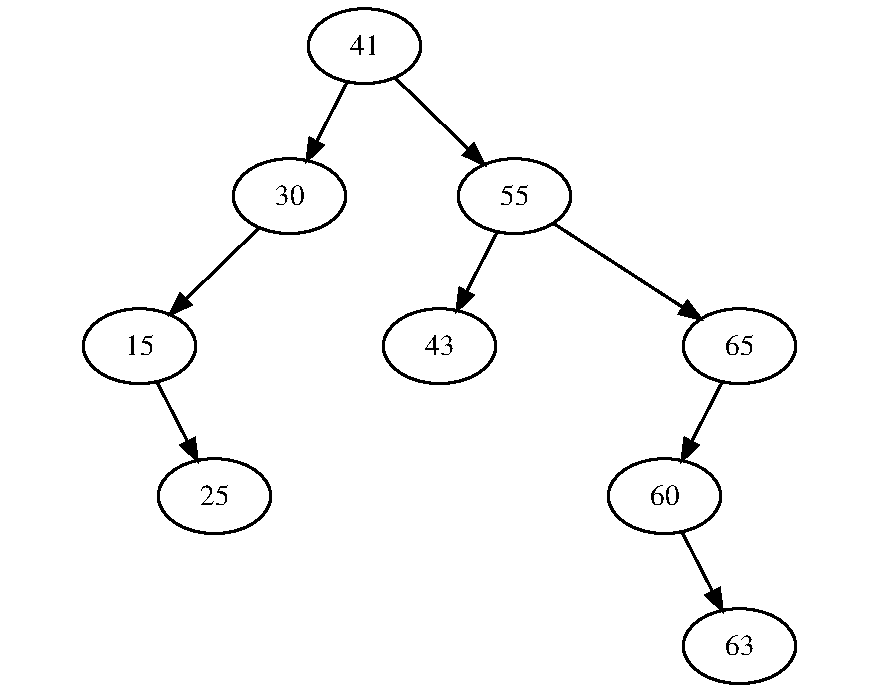
\includegraphics[height=2.5in]{imgs/bst.pdf}
\end{figure}

What is the output of a postorder traversal that, for each visit, prints the {\it depth} of the node?
\begin{choices}	
	\choice None of the others	
	\choice 4, 2, 1, 0, 1, 3, 2, 1, 0	
	\choice 3, 2, 1, 2, 4, 3, 2, 1, 0	
	\choice 3, 2, 1, 2, 3, 3, 1, 1, 0	
	\choice 3, 2, 3, 2, 1, 4, 2, 1, 0
\end{choices}
\answerline

\question[5] 
Indicate the sum of the values corresponding to all statements that are \verb|True|.  Mark $0$ if none are \verb|True|:
\begin{itemize}
	\item[$(1)$] A binary heap is a complete BST
	\item[$(2)$] $2^h$ is the minimum number of nodes in a binary heap of height $h$
	\item[$(4)$] Traversing a BST using {\it pre-order} results in a sorted list of keys
	\item[$(8)$] A binary heap is a complete binary tree\end{itemize}
\answerline

\end{questions}

\end{document}